%!TEX root=../../autopilot.tex
\section{Hardware}
\label{sec:hardware}

The Raspberry Pi can interface with nearly all common hardware, and has an \href{https://www.raspberrypi.org/help/}{extensive collection} of \href{https://elinux.org/RPi_Guides}{guides}, \href{https://elinux.org/RPi_Tutorials}{tutorials}, and an active \href{https://www.raspberrypi.org/forums/}{forum} to support users implementing new hardware. There is also an enormous amount of existing hardware for the Raspberry Pi, including \href{https://www.hifiberry.com/}{sound cards}, \href{https://www.adafruit.com/product/2348}{motor controllers}, \href{https://www.digikey.com/product-detail/en/raspberry-pi/SENSE-HAT/1690-1013-ND/6196429}{sensor arrays}, \href{https://www.seeedstudio.com/Raspberry-Pi-High-Precision-AD-DA-Board-p-2765.html}{ADC/DACs}, and \href{https://www.digikey.com/product-detail/en/pimoroni-ltd/PIM369/1778-1221-ND/9521981}{touchscreen displays}, largely eliminating the need for expensive proprietary hardware (Table \ref{tab:periphs}). 

\begin{margintable}[0.3cm]
\caption{
\textbf{Cost of common peripherals.} The native hardware of the Raspberry Pi and low-level hardware control of Autopilot make most custom-built peripherals unnecessary. While Bpod requires an additional module to decode rotary encoder signals, for example, Autopilot can directly decode them via its GPIO pins with minimal effort by using \href{https://pypi.org/project/pigpio-encoder/}{existing open-source libraries.} Inexpensive off-the-shelf hardware is also available to supplement the Pi's native hardware.}
\label{tab:periphs}
\noindent\begin{tabularx}{\linewidth}{Rll}
\toprule
\textbf{Device} & Raspi & Bpod \\
\midrule
ADC/DAC & \href{https://www.seeedstudio.com/Raspberry-Pi-High-Precision-AD-DA-Board-p-2765.html}{\$30} &  \href{https://sanworks.io/shop/viewproduct?productID=1021}{\$475}/\href{https://sanworks.io/shop/viewproduct?productID=1013}{\$475}\\
I2C & \$0 & \href{https://sanworks.io/shop/viewproduct?productID=1019}{\$165} \\
Ethernet & \$0 & \href{https://sanworks.io/shop/viewproduct?productID=1025}{\$235} \\
Rotary Encoder & \$0 &  \href{https://sanworks.io/shop/viewproduct?productID=1022}{\$135}\\
\bottomrule
\end{tabularx}
\end{margintable}

\begin{marginfigure}[1cm]
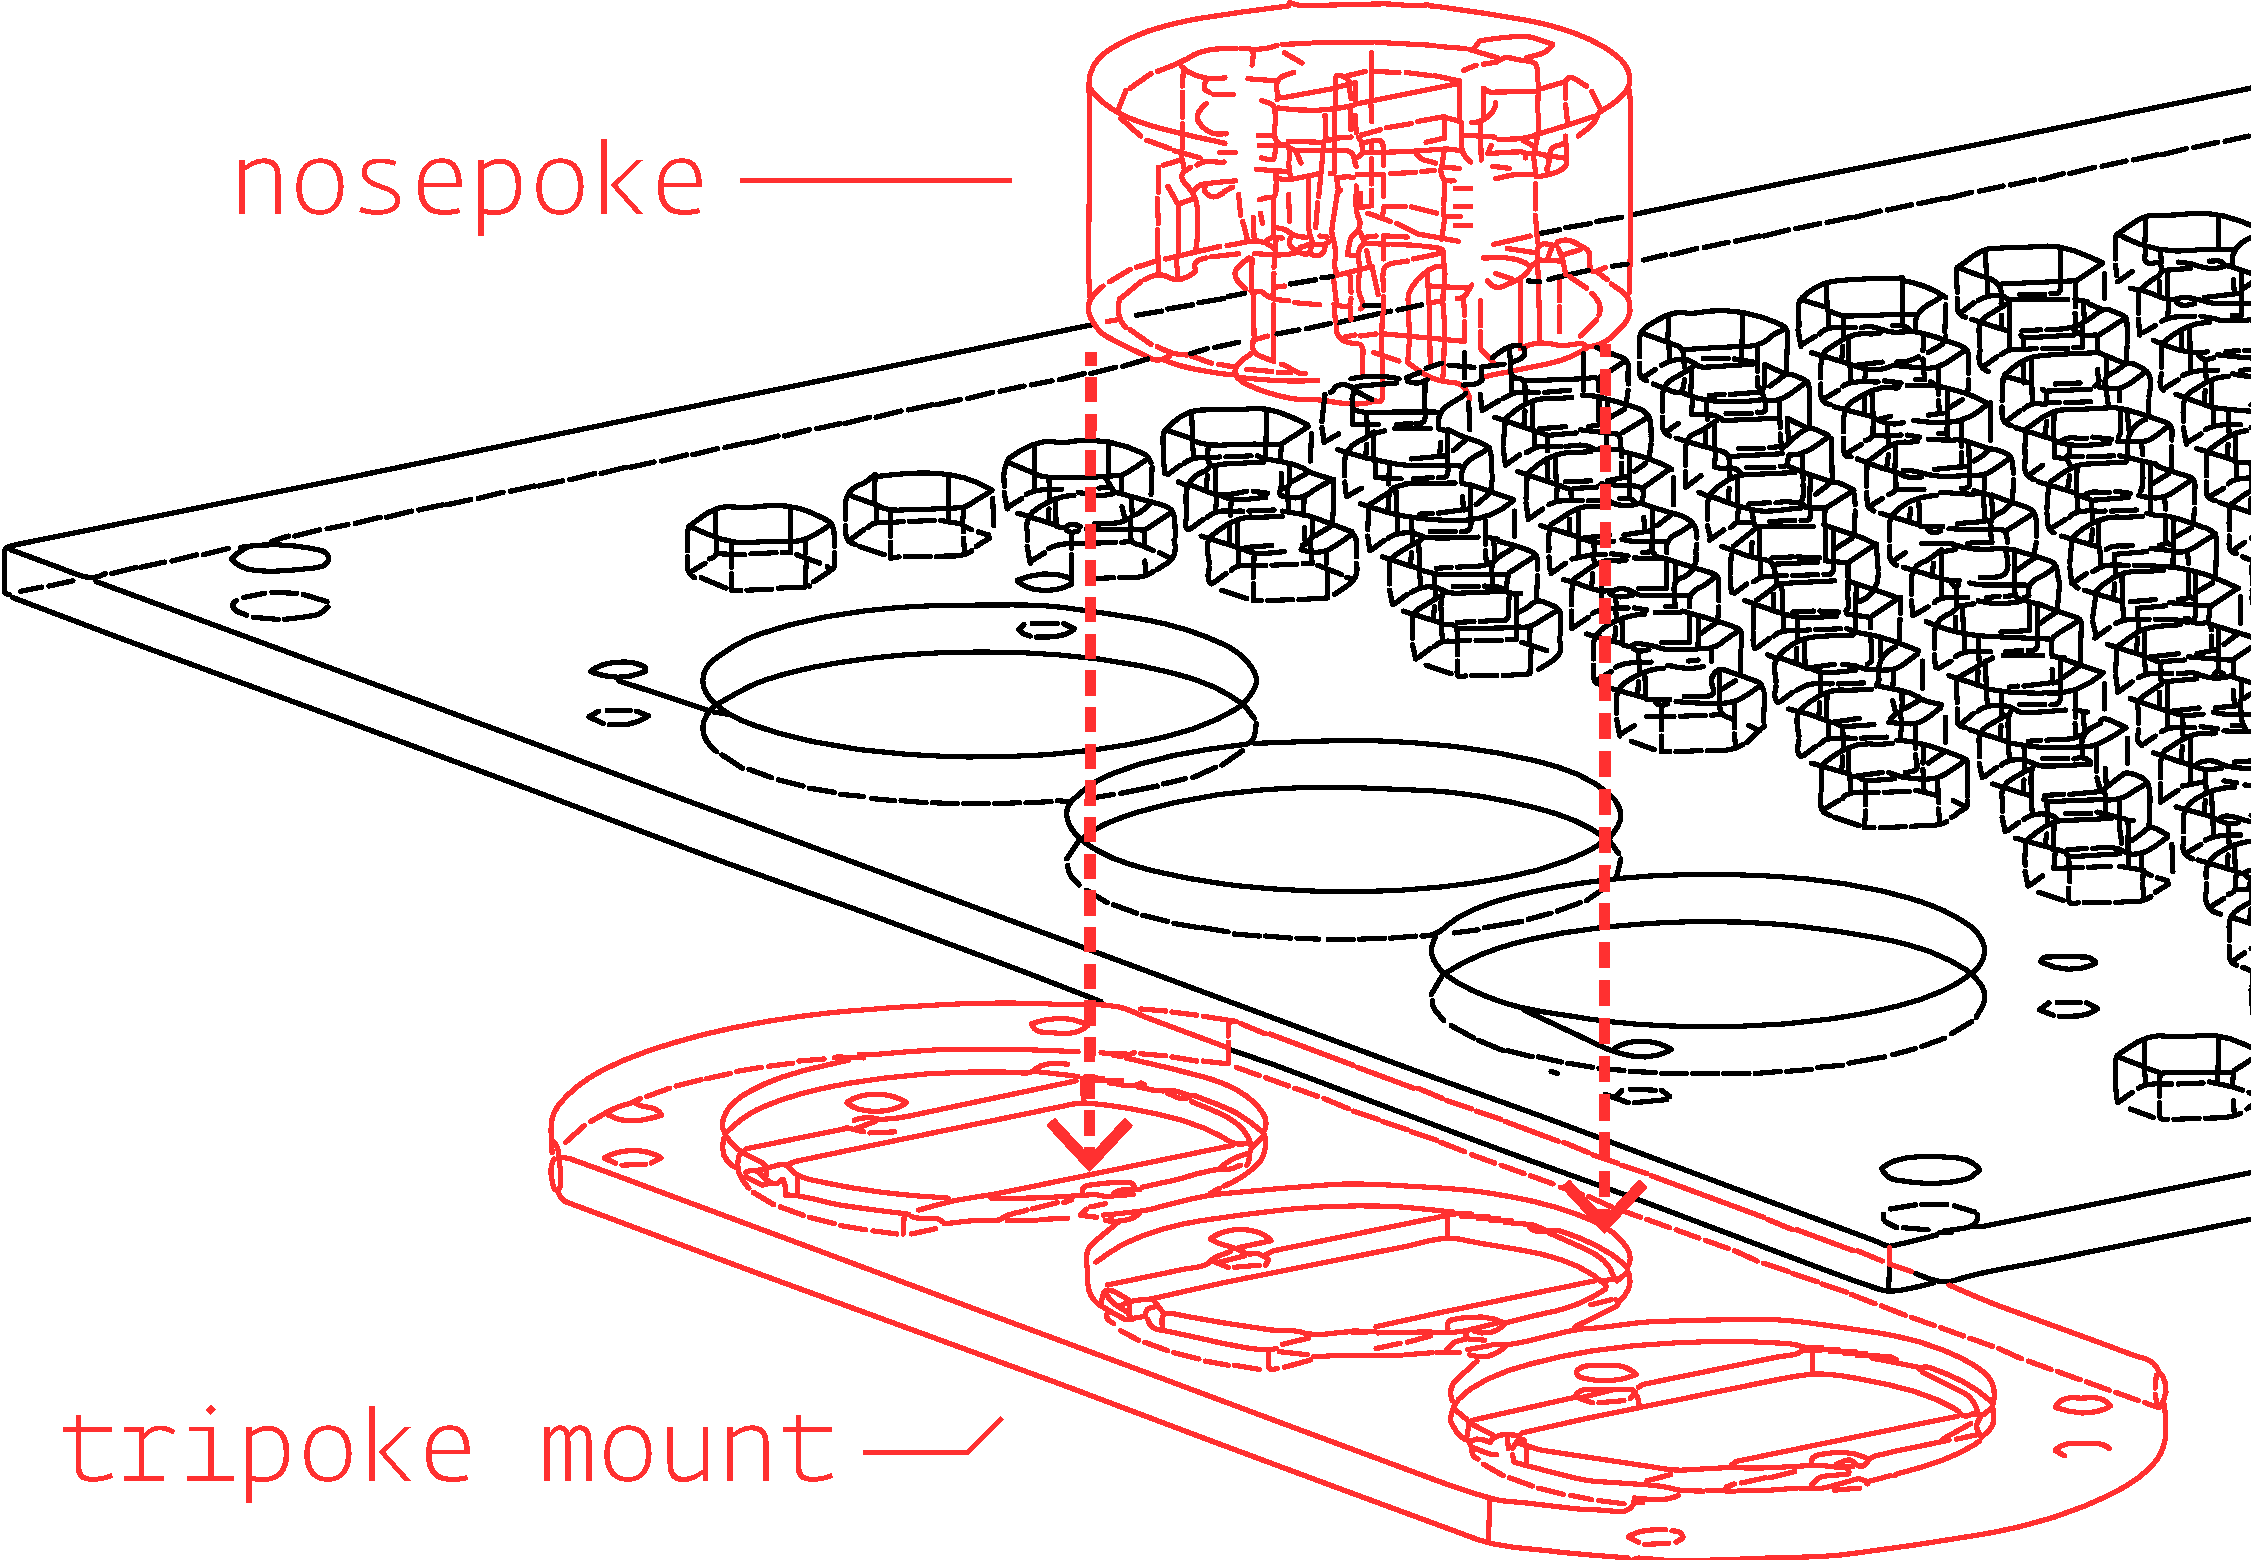
\includegraphics[]{figures/pokeport.pdf}
\caption{We have designed a basic set of easily-assembled hardware available on \href{https://auto-pi-lot.com/hardware/}{Autopilot's website}.}
\label{fig:pokeport}
\end{marginfigure}%

\begin{table*}[b]
\caption{Specifications of reviewed behavior hardware}
\label{hwtab}
\begin{tabularx}{\linewidth}{Rrrr}\toprule
& \href{https://www.raspberrypi.org/products/raspberry-pi-4-model-b/specifications/}{\textbf{Raspberry Pi 4B}} & \href{https://www.pjrc.com/teensy/techspecs.html}{\textbf{Bpod (Teensy 3.6)}} & \href{https://micropython.org/}{\textbf{pyControl (pyboard)}}\\
\midrule
CPU Clock & 1.5GHz & 180MHz & 168MHz \\
CPU Cores & 4 & 1 & 1 \\
CPU Architecture & ARMv8-A, 64-bit & ARMv7E-M 32-bit & ARMv7E-M 32-bit \\
RAM Size & 1, 2, or 4GB & 256KB & 192KB\\
Storage & MicroSD (any size) & 1024KB & 1024KB \\
GPU & Broadcom VideoCore VI & \textcolor{red}{N/A} & \textcolor{red}{N/A} \\
GPIO Pins & 40 & 58 & 29 \\
USB Ports & 2x USB 2.0, 2x USB 3.0  & 2x USB 2.0 & 1x USB 2.0 \\
Ethernet & 1Gbps & 100Mbps & \textcolor{red}{N/A} \\
WiFi & 2.4/5 GHz 802.11 b/g/n/ac & \textcolor{red}{N/A} & \textcolor{red}{N/A} \\
Camera Input & 15-pin Serial Interface & \textcolor{red}{N/A} & \textcolor{red}{N/A} \\
Bluetooth & \checkmark & \textcolor{red}{N/A} & \textcolor{red}{N/A} \\
\end{tabularx}
\end{table*}

Autopilot uses \href{http://abyz.me.uk/rpi/pigpio/}{pigpio} to interact with its GPIO pins, giving Autopilot $5 \mu s$ measurement precision and enabling protocols that require high precision (such as Serial, PWM, and I2C) for nearly all of the pins. Hardware devices in Autopilot are independent Python objects, so their implementation and logic is flexible across installations and tasks. Hardware logic is also reusable, so it doesn't need to be reimplemented for every task, and is intended to be built into a library of hardware objects analogously to tasks.

All hardware objects can be given callback functions to trigger task events, and can be given their own \hyperref[sec:networking]{networking object} to directly send data and receive configuration input. Time-consuming or continuous operations are run in separate threads and don't block task operation. This makes complex hardware logic easy to implement---for example, if one were using flashing LEDs as an aversive stimulus, the flashes could be delivered with a single method call while the next stage in the task is being computed and other hardware input is still being taken.

Though we expect most users will want to make their own or use existing hardware, we have designed a set of 3D-printable components (Figure \ref{fig:pokeport}), and include them along with assembly instructions and parts lists on \href{https://auto-pi-lot.com/hardware/}{Autopilot's website}. 
\clearpage

\subsection{System Adaptability}

\begin{marginfigure}[0.4cm]
\begin{minted}[frame=lines,fontsize=\small]{json}
{
"AGENT": "pilot",
"AUDIOSERVER": "jack",
"DATADIR": "/some/data/dir",
"NAME": "example_pilot",
"PINS": {
    "LEDS": {
        "C": [22,18,16],
        "L": [11,13,15],
        "R": [19,21,23]}
},
"MSGPORT": 5565,
"TERMINALIP": "192.168.0.100"
}
\end{minted}
\caption{The prefs.json file stores durable system configuration options.}
\label{fig:prefs}
\end{marginfigure}%

Rather than attempting to enforce a uniform hardware ecosystem, Autopilot adapts to the radically divergent hardware of different researchers by keeping hardware logic independent from the way it is set up in a particular system. A systemwide \mintinline{python}{prefs.json} file contains all durable configuration information for your setup (Figure \ref{fig:prefs}). Hardware is then accessed by its type and name, so if a task needs an LED named "C" (for "Center"), it would connect to the pins defined in  \mintinline{python}{prefs['PINS']['LEDS']['C']} no matter how the LED was connected or configured in the system. This layer of abstraction allows the task classes to be general enough to maintain a shared task library while also allowing researchers to retain total control over their system. 
 
Autopilot also allows the hardware in your particular setup to be used for multiple tasks that may have differing hardware demands. We think a common use-case will be a series of mostly-static behavioral boxes that can be reconfigured without being wholly rebuilt. The hardware schematics we release are modular, so that one could, for example, change a behavior box from a freely-moving two-alternative forced choice task to a head-fixed version by replacing a panel and installing a running wheel. We are working to implement support for multiple hardware configurations that can be kept in the \texttt{prefs.json} file and automatically swapped depending on the task being run.